\documentclass[12pt]{article}
\usepackage[utf8]{inputenc}
\usepackage[spanish]{babel}
\usepackage{amsmath}
\usepackage{amsthm}
\usepackage{multicol,multienum}
\usepackage{graphicx}
\usepackage{float}
\usepackage{tikz}
\usepackage{color}
\usepackage{anysize}
\usepackage{anyfontsize}
%Este paquete permite manejar los encabezados del documento
\usepackage{fancyhdr}
%hay que definir el ambiente de la página
\pagestyle{fancy}
%aqui va el texto para todas las paginas l--> izquierda, r--> derecha, hay un C--> para centrar el texto deseado
%\lhead{Curso de Física Computacional}
\fancyhead[R]{\nouppercase{\leftmark}}
%define el ancho de la linea que separa el encabezado del cuerpo del texto
\renewcommand{\headrulewidth}{0.5pt}
\usepackage{hyperref}
%esta parte define el color del marco que aparece en las hiperreferencias.
\definecolor{links}{HTML}{2A1B81}
\hypersetup{colorlinks,linkcolor=,urlcolor=links}
\spanishdecimal{.}
\marginsize{1.5cm}{1.5cm}{2cm}{2cm}
\author{M. en C. Gustavo Contreras Mayén.}
\title{Instalación de Anaconda y Python \\ \begin{Large} Curso de Física Computacional\end{Large} \\
\begin{small}
\texttt{curso.fisica.comp@gmail.com}
\end{small}}
\date{ }
\begin{document}
\maketitle
\fontsize{14}{14}\selectfont
En el curso de Física Computacional manejaremos \texttt{Python} como lenguaje de programación, por lo que será necesario contar con un equipo de cómputo para trabajar fuera del laboratorio; a continuación presentamos una guía breve de la instalación de \texttt{Python} en un equipo que opere con Linux o Windows.
\\
\\
La distribución de Anaconda con \texttt{Python} permite la instalación del kernel además de un conjunto de paquetes en un sólo paso al momento de instalar, otra manera de contar con el mismo entorno de Anaconda, sería instalar paquete por paquete, pero hay que tomar en cuenta que un paquete puede requerir de otro (dependencia) y antes de instalar ese paquete, habría que instalar otro(s) inicialmente. La distribución de Anaconda resuelve todo esto y nos evita los conflictos en caso de requerir las dependencias.
\\
\\
Anaconda cuenta con paquetes de instalación para los sistemas operativos Windows, Linux y Mac, en el caso de Windows, hay que revisar la versión del sistema operativo, es decir, si es de 32 o 64 bits, esto es importante dado que optimizamos el uso del procesador en el caso de 64 bits. A continuación veremos de manera gráfica el proceso de instalación de Anaconda bajo Windows.
\section{Instalando Anaconda en Windows.}
Podemos utilizar \texttt{Python} y las librerías más comunes a partir de una instalación sucesiva de los archivos, requiere que conozcamos la versión del sistema operativo que tengamos en nuestro equipo. Comencemos con una instalación bajo Windows.
\begin{enumerate}
\item Hay que descargar de la página de Anaconda: \url{http://continuum.io/downloads}, la versión de nuestro sistema operativo\footnote{En este ejemplo, la instalación se revisa en un equipo con Windows 7 @ 32 bits.}.
\item Hacemos doble click sobre el archivo que se descargó para iniciar el proceso de instalación.
\begin{figure}[H]
	\centering
	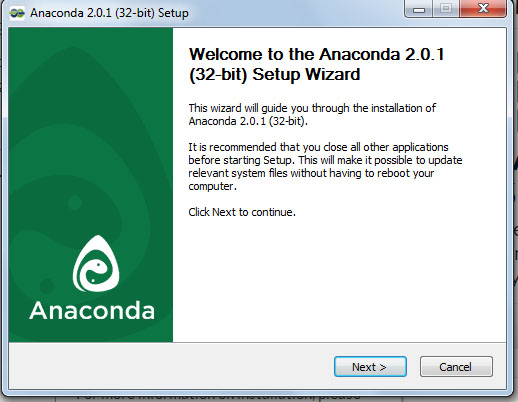
\includegraphics[scale=0.5]{Imagenes/Instalacion_Anaconda_01.jpg} 
\end{figure}
\item Se acepta la licencia de uso de la distribución.
\begin{figure}[H]
	\centering
	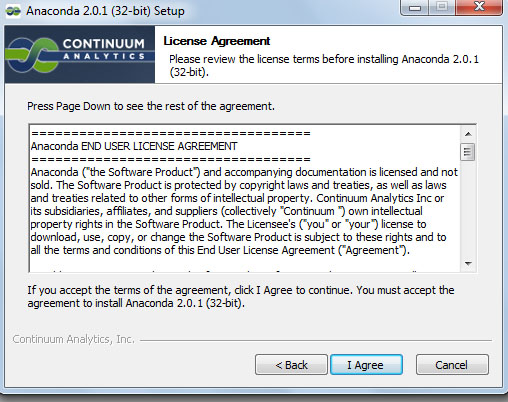
\includegraphics[scale=0.5]{Imagenes/Instalacion_Anaconda_02.jpg} 
\end{figure}
\item En el caso de que tu equipo bajo Windows tenga varios usuarios, hay que definir si se permite la ejecución para todos los usuarios o sólo para el que está realizando la instalación, Anaconda recomienda que sea sólo al usuario que instala.
\begin{figure}[H]
	\centering
	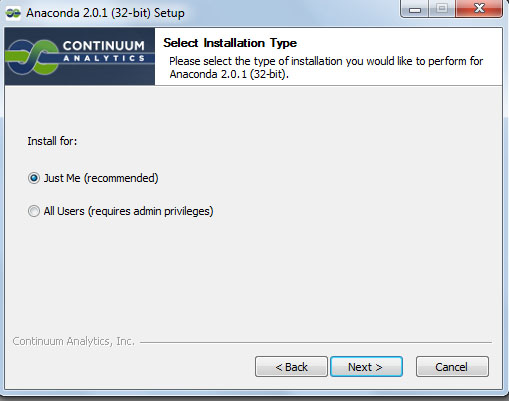
\includegraphics[scale=0.5]{Imagenes/Instalacion_Anaconda_03.jpg} 
\end{figure}
\item Las carpetas de instalación se manejan por defecto, se recomiend no modificar la ruta.
\begin{figure}[H]
	\centering
	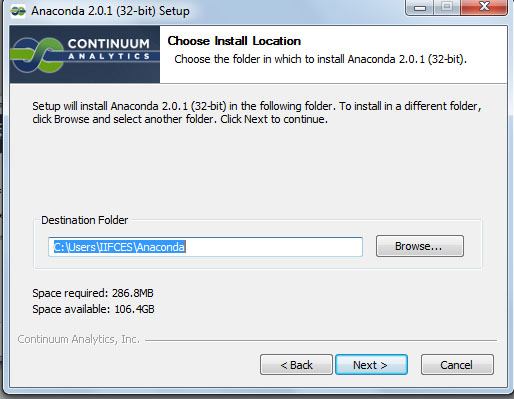
\includegraphics[scale=0.5]{Imagenes/Instalacion_Anaconda_04.jpg} 
\end{figure}
\item Opciones de instalación avanzadas:
\begin{enumerate}
\item Agregar Anaconda al PATH como Entorno de Variable. Esto permite que podamos ejecutar \texttt{Python} desde cualquier ruta dentro de nuestro equipo, es decir, no necesitaremos cambiar de carpeta para localizar al ejecutable de \texttt{Python}, por lo que dejamos la marca.
\item Registrar Anaconda como programa para \texttt{Python 2.7}. Asocia la ejecución de archivos \texttt{*.py} con la distribución Anaconda.
\end{enumerate}
\begin{figure}[H]
	\centering
	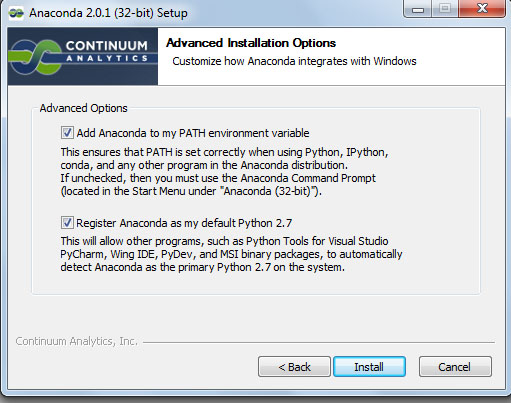
\includegraphics[scale=0.5]{Imagenes/Instalacion_Anaconda_05.jpg} 
\end{figure}
\item Conforme se realice la instalación, veremos una barra con el avance.
\begin{figure}[H]
	\centering
	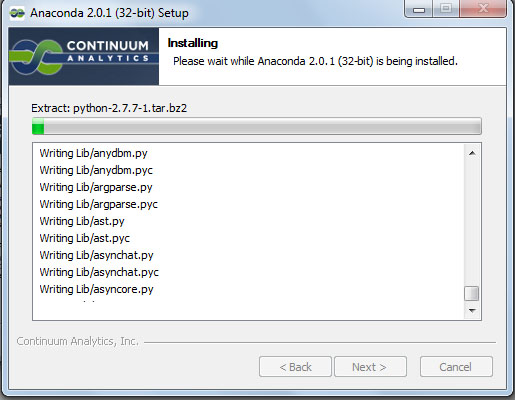
\includegraphics[scale=0.5]{Imagenes/Instalacion_Anaconda_06.jpg} 
\end{figure}
\item Una vez que se completó la instalación, se habilita el botón Siguiente.
\begin{figure}[H]
	\centering
	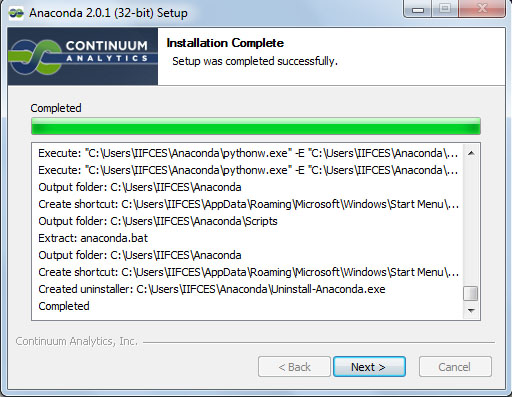
\includegraphics[scale=0.5]{Imagenes/Instalacion_Anaconda_07.jpg} 
\end{figure}
\item Con la instalación completa ya tenemos disponible y listo para usar en nuestro equipo Anaconda.
\begin{figure}[H]
	\centering
	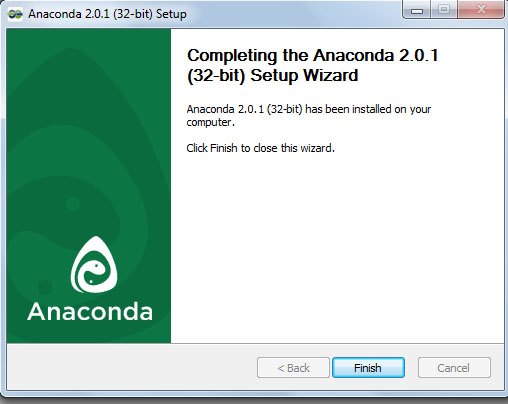
\includegraphics[scale=0.5]{Imagenes/Instalacion_Anaconda_08.jpg} 
\end{figure}
\item En el menú de Windows podemos localizar la carpeta que se asoció a los programas de Anaconda.
\begin{figure}[H]
	\centering
	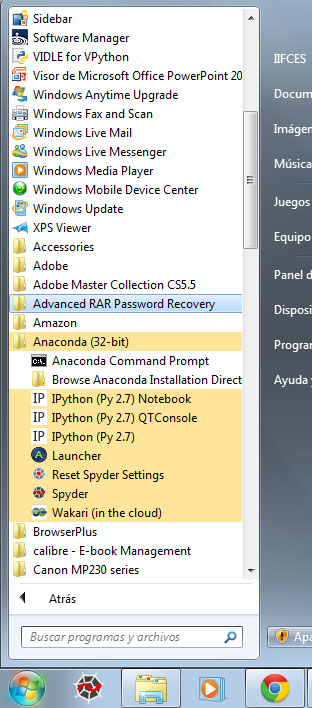
\includegraphics[scale=0.5]{Imagenes/Instalacion_Anaconda_09.jpg} 
\end{figure}
\item Podemos ejecutar la ventana de comandos de Anaconda para llamar a \texttt{Python}, una vez abierta la ventana, tecleamos \texttt{python}, y veremos la versión que se ha instalado en nuestro equipo.
\begin{figure}[H]
	\centering
	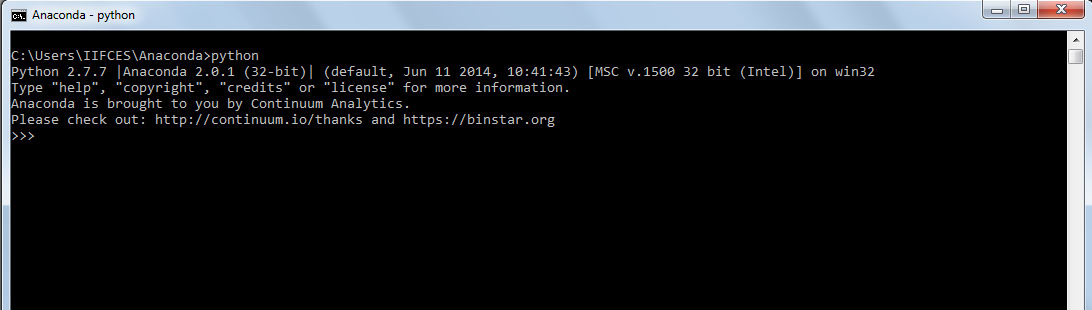
\includegraphics[scale=0.5]{Imagenes/Instalacion_Anaconda_10.jpg} 
\end{figure}
Esto completa el proceso de instalación de Anaconda y \texttt{Python} en nuestro equipo.
\end{enumerate}
\section{Instalando Anaconda en Mac.}
Al igual que en Windows podemos utilizar \texttt{Python} y las librerías más comunes a partir de una instalación sucesiva de los archivos, de hecho en el link que se ofrece cuenta con la opción miniconda que permite realizar estas acciones, el procedimiento descrito es mediante ayuda gráfica. 
\begin{enumerate}
\item Hay que descargar de la página de Anaconda: \url{http://continuum.io/downloads}, la versión de nuestro sistema operativo\footnote{En este ejemplo, la instalación se revisa en un equipo con MacOsx 7.5}, la imagen muestra como se ve la pantalla de ingreso y las opciones que trae el instalador.
\begin{figure}[H]
	\centering
	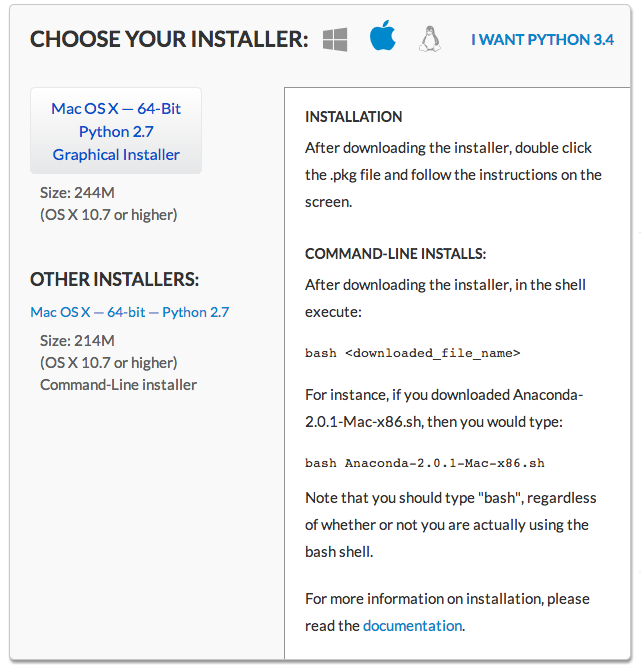
\includegraphics[scale=0.5]{Imagenes/instalacion} 
\end{figure}
\item Seleccionando la opción de "Graphical Installer" se ejecutará la descarga de un archivo, una vez completada la descarga se da doble click sobre el mismo, esto desplegará un menú como el mostrado en la siguiente figura.
\begin{figure}[H]
	\centering
	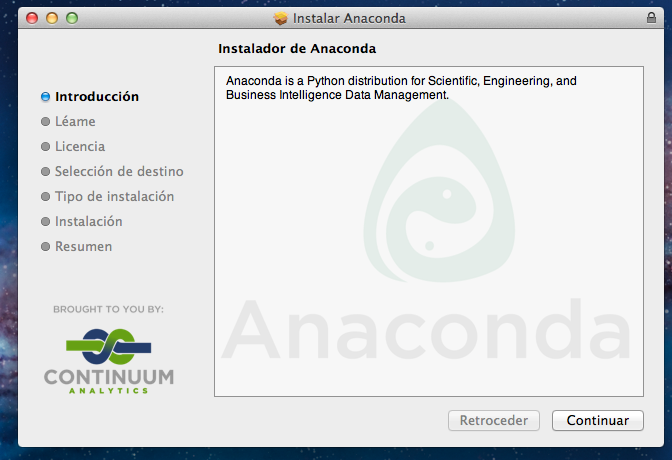
\includegraphics[scale=0.5]{Imagenes/instalacion1} 
\end{figure}
\item Se da continuar hasta llegar a la opción de aceptar la licencia de uso de la distribución, se da continuar y aparecerá una pantalla que demanda aceptar la licencia.
\begin{figure}[H]
	\centering
	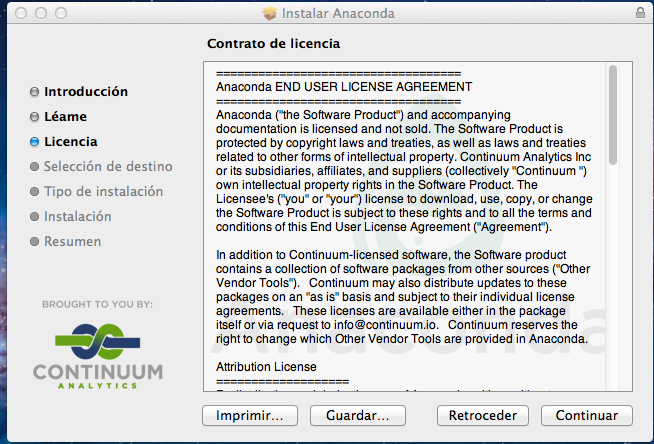
\includegraphics[scale=0.5]{Imagenes/instalacion2} 
\end{figure}
\item Las carpetas de instalación se manejan por defecto, se recomienda no modificar la ruta.
\begin{figure}[H]
	\centering
	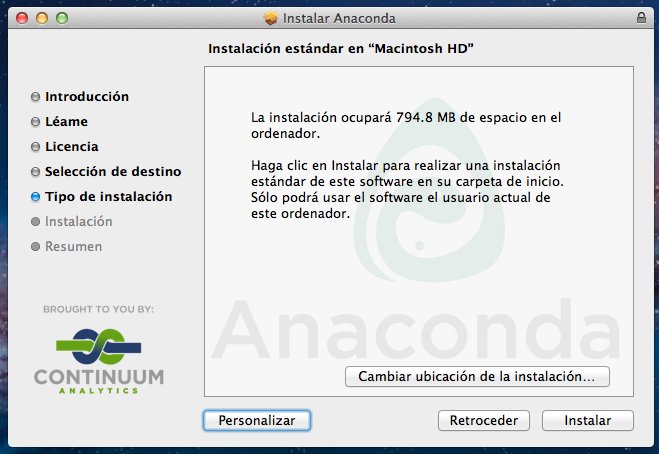
\includegraphics[scale=0.5]{Imagenes/instalacion3} 
\end{figure}
\item Una vez que se completó la instalación, se muestra en pantalla lo siguiente, paralelamente se instala un icono en el escritorio como el que se muestra en la figura  contigua.
\begin{figure}[H]
	\centering
	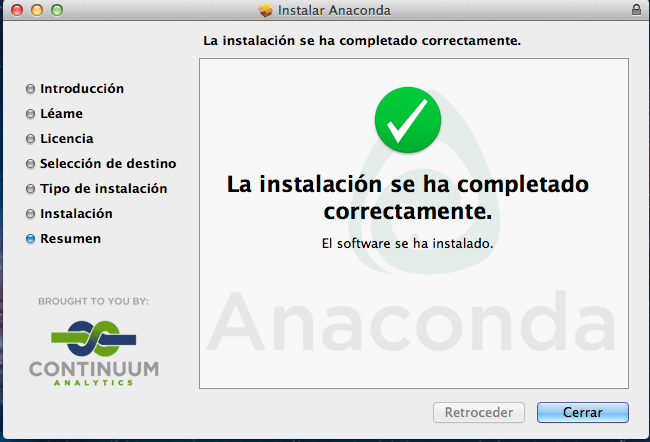
\includegraphics[scale=0.5]{Imagenes/instalacion4} 
\end{figure}
\begin{figure}[H]
	\centering
	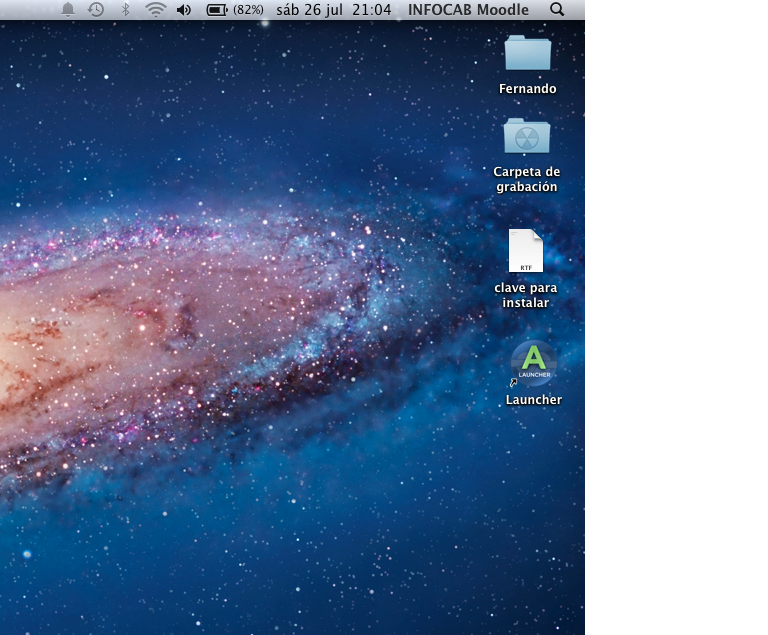
\includegraphics[scale=0.4]{Imagenes/laun} 
\end{figure}  
\item Con la instalación completa debemos dar doble click sobre el mismo icono esto desplegará un menú como el que se muestra en la imagen.
\begin{figure}[H]
	\centering
	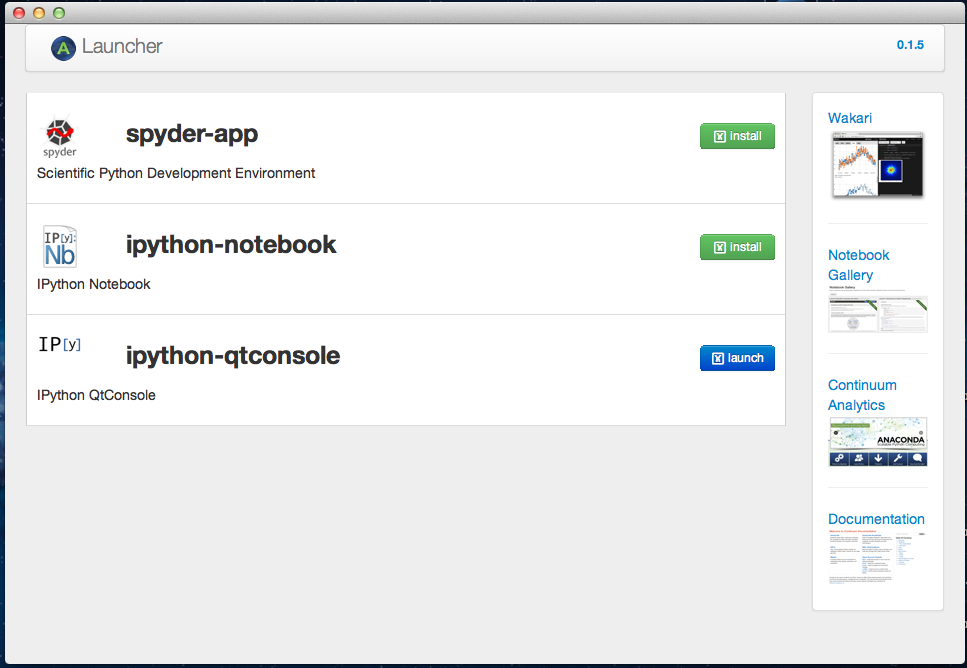
\includegraphics[scale=0.5]{Imagenes/instalacion6} 
\end{figure}
\item En el menú se van dando click sobre Install, el sistema te pedirá esperar y al finalizar la opción cambiará Launch.
\item Podemos ejecutar la ventana de comandos de Anaconda para llamar a \texttt{iPython-notebook}, una vez abierta la ventana, ya se tiene la terminal de \texttt{Python} lista para trabajar en modo rudo.
\begin{figure}[H]
	\centering
	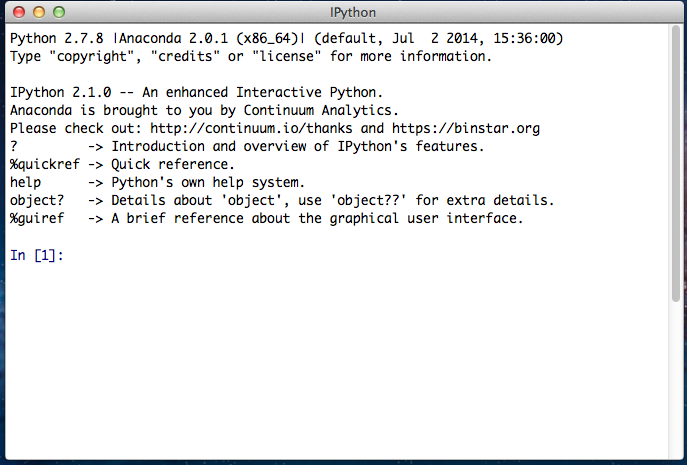
\includegraphics[scale=0.5]{Imagenes/instalacion7} 
\end{figure}
\end{enumerate}
\section{Instalando Anaconda en Linux}
La instalación de Anaconda en Linux (en este ejemplo se usa Ubuntu como distribución de linux) se puede realizar de dos modos: con Synaptic o directamente con el archivo.
\\
\\
Veremos el caso de  la instalación con el paquete que se descarga de la página oficinal de Anaconda.
\begin{enumerate}
\item El primer paso es descargar la versión que corresponda con nuestra distribución de linux, ya sea de 32 bits o 64 bits
\begin{figure}[H]
	\centering
	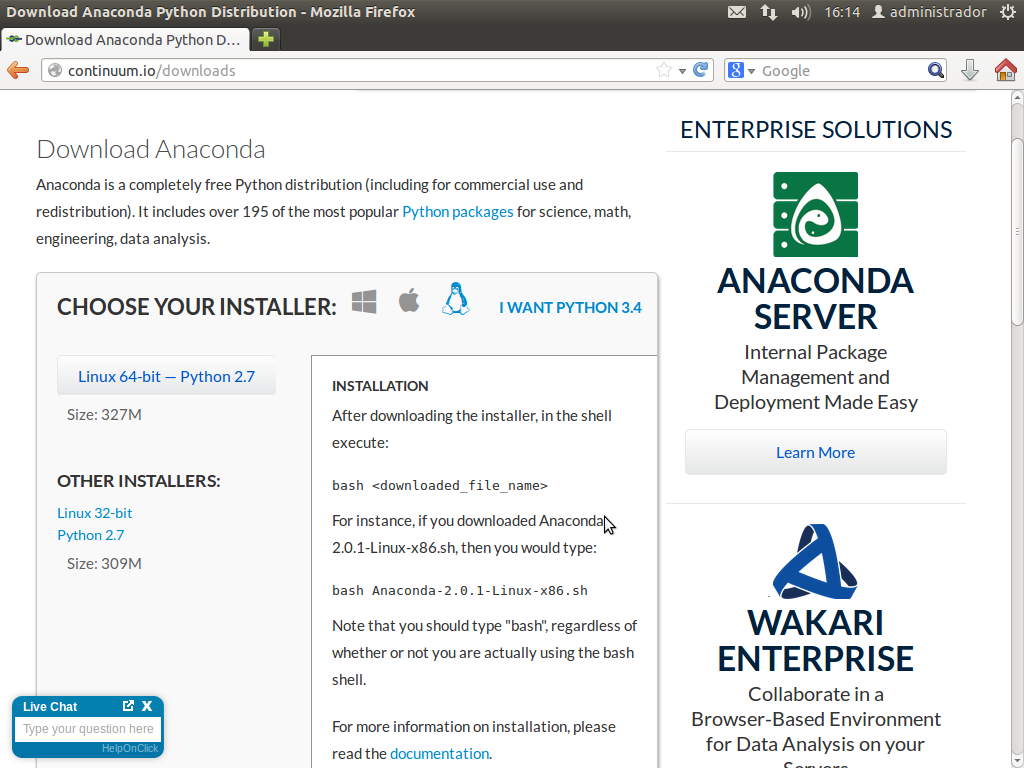
\includegraphics[scale=0.35]{Imagenes/Anaconda_Linux_01.png} 
\end{figure}
\item El siguiente paso es descargar el archivo en el equipo
\begin{figure}[H]
	\centering
	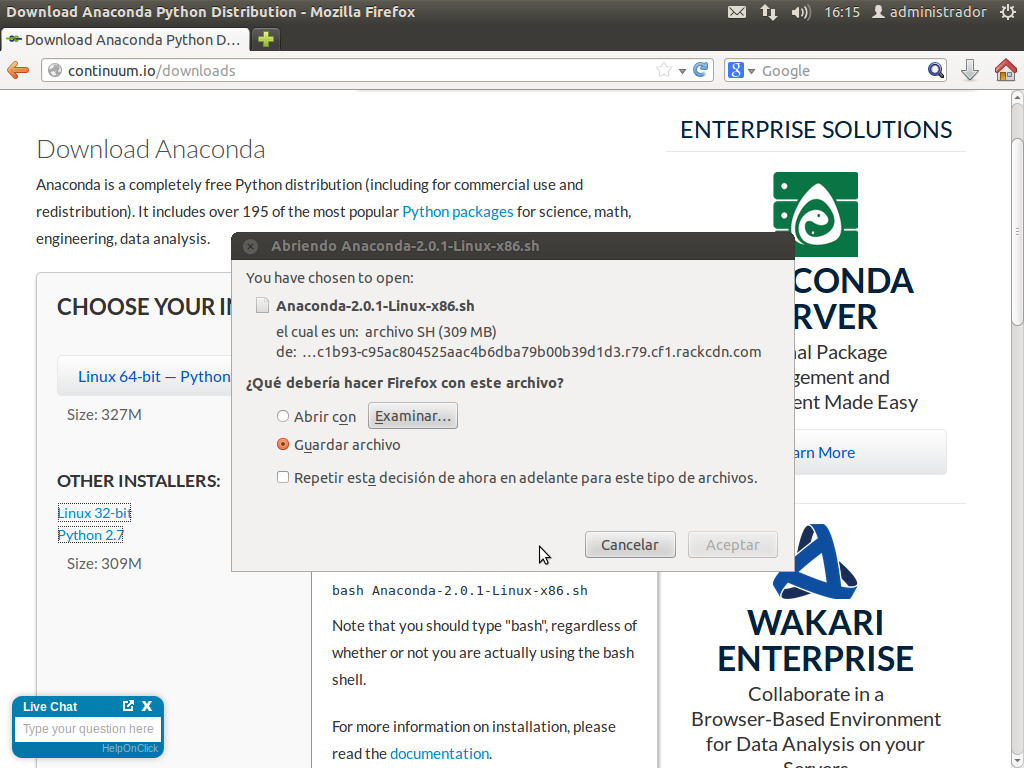
\includegraphics[scale=0.35]{Imagenes/Anaconda_Linux_02.png} 
\end{figure}
\item De acuerdo a la documentación de Anaconda, abrimos una terminal de linux y tecleamos el comando
\\
\begin{verbatim}
bash Anconda-2.0.1-Linux-x86.xh
\end{verbatim}
Toma en cuenta que el nombre del archivo que has descargado, puede ser diferente, por ello verifica antes de teclear el comando.
\begin{figure}[H]
	\centering
	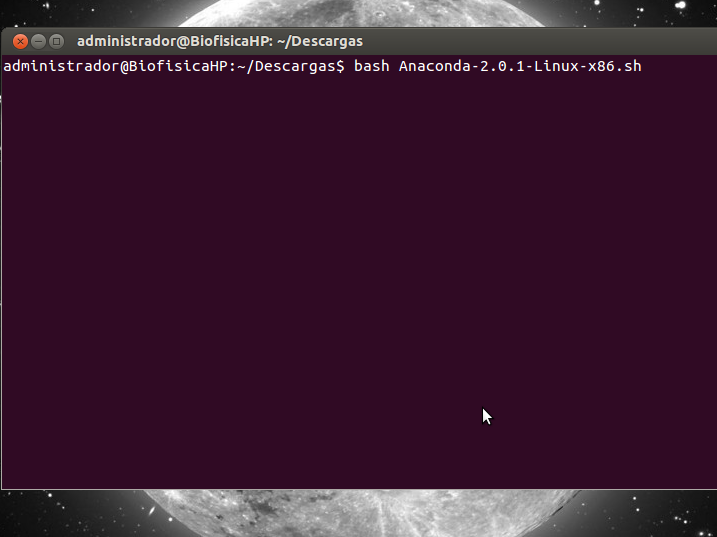
\includegraphics[scale=0.5]{Imagenes/Anaconda_Linux_03.png} 
\end{figure}
\item Para iniciar la instalación en nuestro equipo, basta con que tecleemos \texttt{Enter}, y se inicie el proceso.
\begin{figure}[H]
	\centering
	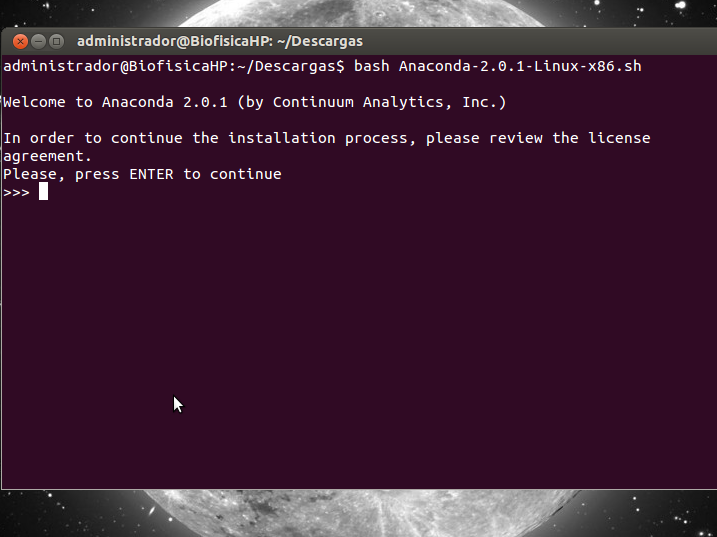
\includegraphics[scale=0.5]{Imagenes/Anaconda_Linux_04.png} 
\end{figure}
\item Recomendamos altamente que no se modifiquen la ruta de instalación, por lo que tecleamos \texttt{Enter} para aceptar la ruta por defecto, en caso de que decidas modificar la ruta de instalación, posteriormente para ligar los paquetes que se descarguen, deberás de hacer ajustes de manera manual y por cada paquete que instales, por ello, es conveniente manejar la ruta que nos indica Anaconda.
\begin{figure}[H]
	\centering
	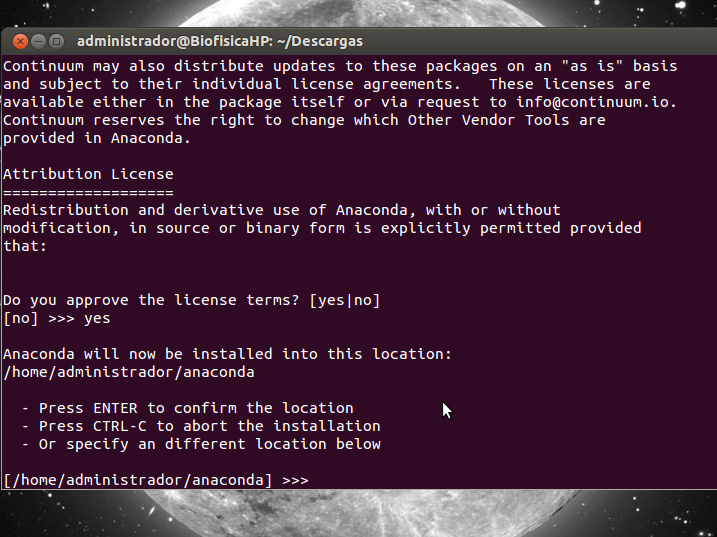
\includegraphics[scale=0.5]{Imagenes/Anaconda_Linux_05.png} 
\end{figure}
\item Veremos en la terminal, la instalación de los paquetes de manera automática. Una ventaja de usar una plataforma como Anaconda es que los programas, paquetes y librerías ya llevan las referencias necesarias, en caso de que se haga una instalación por separado de cada elemento, lo más seguro es que se requieran y se resuelvan las dependencias necesarias, proceso que puede ser muy tedioso.
\begin{figure}[H]
	\centering
	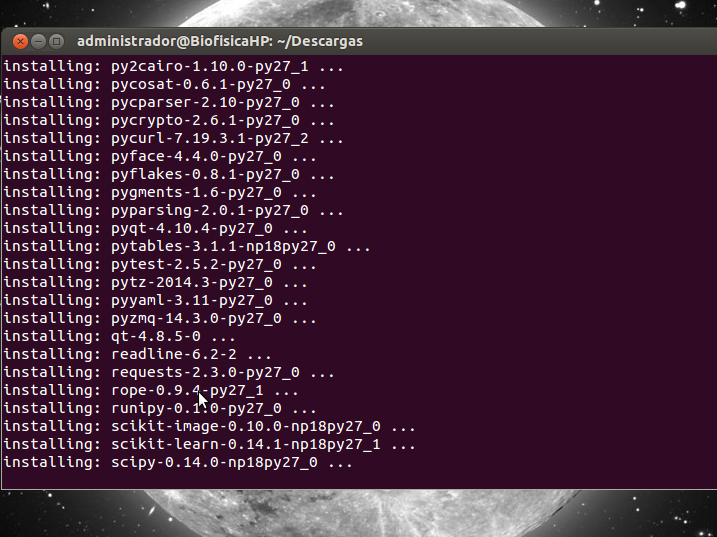
\includegraphics[scale=0.5]{Imagenes/Anaconda_Linux_06.png} 
\end{figure}
\item Para configurar la ejecución de \texttt{Python} desde cualquier punto, hay que ajustar el \texttt{PATH} en el respectivo archivo de linux, por lo que aceptamos el ajuste al archivo.
\begin{figure}[H]
	\centering
	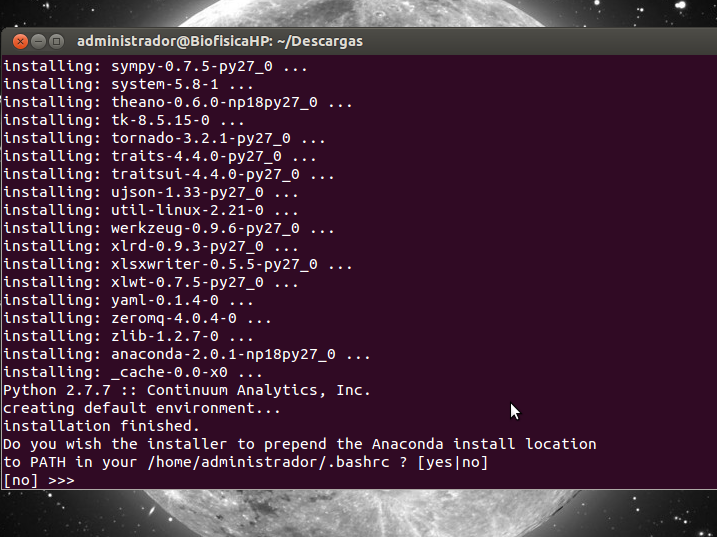
\includegraphics[scale=0.5]{Imagenes/Anaconda_Linux_07.png} 
\end{figure}
\item El proceso de instalación, prácticamente concluye con el paso anterior, por lo que verificamos que ya tenemos instalado \texttt{Python} en nuestro equipo, dentro de la terminal escribimos \texttt{python} y debemos de visualizar el encabezado del programa y debemos de notar que el prompt ya cambió al símbolo $>>>$
\begin{figure}[H]
	\centering
	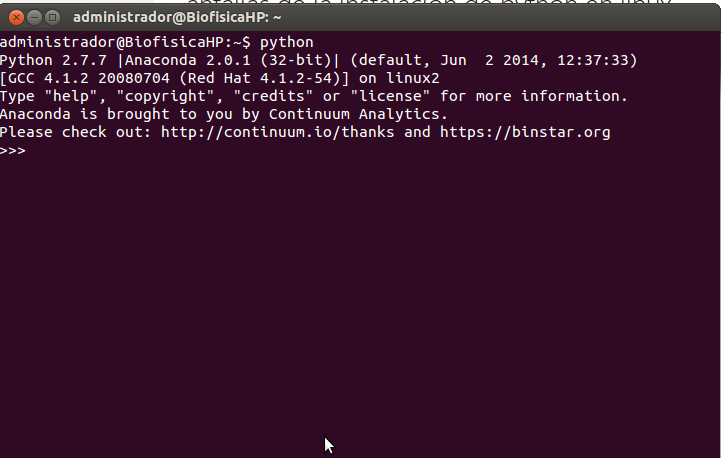
\includegraphics[scale=0.5]{Imagenes/Anaconda_Linux_08.png} 
\end{figure}
\end{enumerate}

\end{document}